\section{Proposta de trabalho}
\subsection{Objetivos}
\begin{frame}{Objetivo}
    \begin{block}{Objetivo geral}
    Propor uma estratégia para verificação formal para aprimoramento de segurança aplicada na fase de pré-implementação de CIs escritos em \textbf{Solidity} para detecção das vulnerabilidades de \textbf{reentrância}, \textbf{\textit{delegatecall injection}} e \textbf{contrato suicida}, por meio da técnica de \textbf{\textit{model checking}}.
    \end{block}
    Objetivos específicos:
    \begin{itemize}
        \item Determinar o formalismo adequado para modelagem dos contratos e para representação das vulnerabilidades;
        \item Implementar o método de verificação;
        \item Definir as estratégias para validação da proposta.
    \end{itemize}
\end{frame}

\begin{frame}{Proposta}
    \begin{block}{}
    Framework para verificação formal de CIs escritos em Solidity na fase de pré-implantação.
    \end{block}
    Tarefas realizadas por meio do framework:
    \begin{itemize}
        \item Inclusão do código fonte em Solidity;
        \begin{itemize}
            \item Pode ser mais de um;
            \item Relações intercontratuais;
            \item Diagrama de fluxo de interação entre CIs.
        \end{itemize}
        \item Conversão do código para modelo de estados;
        \item Exibição do modelo obtido;
        \item Inserção das propriedades e seleção das vulnerabilidades;
        \begin{itemize}
            \item Modelo para descrição;
            \item Mais próximo de linguagem natural.
        \end{itemize}
    \end{itemize}
\end{frame}

\begin{frame}{Proposta}
    \begin{block}{}
    Framework para verificação formal de CIs escritos em Solidity na fase de pré-implantação.
    \end{block}
    Tarefas realizadas por meio do framework:
    \begin{itemize}
        \item Conversão para lógica temporal;
        \item Verificação;
        \item Exibição dos resultados.
        \begin{itemize}
            \item Indicação das vulnerabilidades no código.
        \end{itemize}
    \end{itemize}
\end{frame}

\begin{frame}{Proposta}
    \begin{block}{}
    Framework para verificação formal de CIs escritos em Solidity na fase de pré-implantação.
    \end{block}
    Validação: 
    \begin{itemize}
        \item Experimento sobre um conjunto de CIs com vulnerabilidades já conhecidas;
        \item Avaliar a eficácia e acurácia da verificação;
        \item Eficiência;
        \begin{itemize}
            \item Consumo de memória, processamento e tempo de execução.
        \end{itemize}
    \end{itemize}
    Estudo de caso:
    \begin{itemize}
        \item Aplicado para tratar de propriedades funcionais relativas aos requisitos do CI.
    \end{itemize}    
\end{frame}

\begin{frame}{Framework proposto}
    \begin{figure}[!htb]
     \centering
     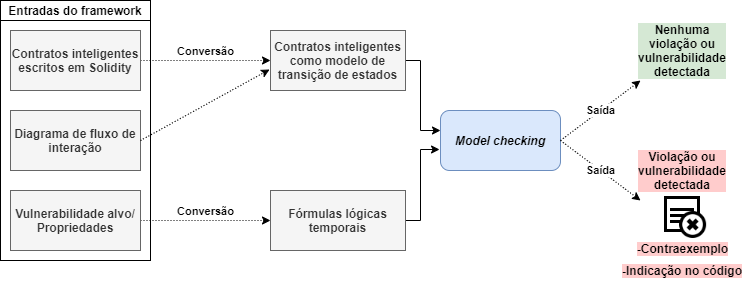
\includegraphics[scale=0.4]{figuras/proposta/framework.png}
    \end{figure}    
\end{frame}

\subsection{Trabalhos relacionados}
\begin{frame}{O framework de Mavridou et al. (2019)}
    \begin{itemize}
    	\item Framework VeriSolid;
    	\item Modelagem gráfica dos CIs como máquina de estados finito (MEF);
    	\item Extensão do framework FSolidM, de Mavridou e Laszka (2018);
    	\item MEF $\rightarrow$ Código Solidity;
    	\begin{itemize}
    		\item Erros evitados direto na construção.
    	\end{itemize}
    	\item Baseada na MEF, propriedades podem ser especificadas;
    	\item Não é abordada nenhuma vulnerabilidade específica.
    \end{itemize}
\end{frame}

\begin{frame}{O framework de Nelaturu \textit{et al.} (2020)}
	\begin{itemize}
		\item Extensão do VeriSolid;
		\item Permite a relação entre múltiplos contratos;
		\begin{itemize}
			\item Diagrama de implementação.
		\end{itemize} 
		\item Implantação do automática dos CIs gerados;
		\item Vulnerabilidades de reentrância e exceções não tratadas;
		\begin{itemize}
			\item Prevenidas na construção de MEF.
		\end{itemize}
		\item Vulnerabilidades de endereço curto, contrato suicida e bloqueio de Ether;
		\begin{itemize}
			\item Verificadas na modelagem ou implantação.
		\end{itemize}
		\item Propriedades descritas por meio de \textit{templates} em linguagem natural;
		\item Reentrância:
		\begin{itemize}
			\item Não permite a execução de funções \textit{callback};
			\item Desconsidera casos onde a função é usada sem causar, necessariamente, uma vulnerabilidade.
		\end{itemize}
	\end{itemize}
\end{frame}

\begin{frame}{Framework proposto}
	Proposta do trabalho:
	\begin{itemize}
		\item Relações intercontratuais: Diagrama de fluxo de interação;
		\item Modelagem de funções \textit{callback};
		\item \textit{Delegatecall injection}:
		\begin{itemize}
			\item Não é abordada em nenhum trabalho por meio do \textit{model checking}.
		\end{itemize}
		\item Apontamento das vulnerabilidades no código;
		\item Tarefas manuais:
		\begin{itemize}
			\item Especificação e seleção das vulnerabilidades/propriedades;
			\item Diagrama de fluxo de interação.
		\end{itemize}
	\end{itemize}
\end{frame}

\subsection{Plano de trabalho}
\begin{frame}{Plano de trabalho}
    \begin{figure}[ht]
    \centering
    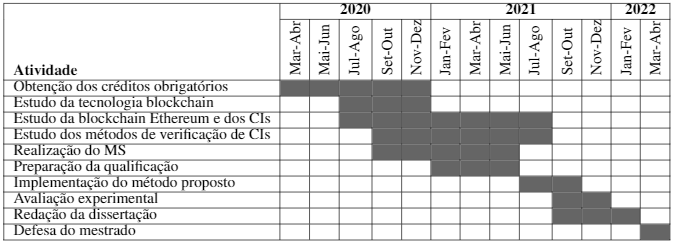
\includegraphics[width=10cm]{figuras/proposta/plano_de_trabalho.png}
    \end{figure}
\end{frame}
